The MPI implementation of the Needleman-Wunsch algorithm uses a Master-Slave paradigm. \\
The master process is in charge of distributing the jobs to the slaves processes. However, the job scheduling is not dynamic : for each diagonal, the master distributes the jobs according to the same pattern. For pratical purposes, the master thread is computing the first tile.
\begin{figure}[htp]
\centering
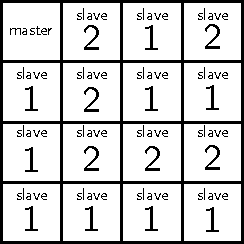
\includegraphics[scale=1.00]{/home/matthieu/Documents/melbourne/cours/parallel_prog/git/nw_parallel/report/fig/mpi1.pdf}
\caption{Scheduling for -np 3 (2 slaves and 1 master)}
\label{}
\end{figure}
\\
One of drawbacks of this technique is that some slaves processes can be waiting for others. But since the tile size is the same for every slave, the workload should be similar among slaves. \\
